%Outline
%%Exectution model
%   *Define what is a OpenSHMEM program: a set of processes (either SPMD or MIMD?) where each process has its own 'local' (private) memory and symmetric memory regions that may be accessible by any PEs.
%   *Each OpenSHMEM process is called a processing element (PE)
%   *Each PE may be mapped to many to one hardware cores/threads or less.
%   *The number of PEs is specified at launch/runtime.
%   *Each PE must call startpe to initialize the OpenSHMEM runtime, before any other call for OpenSHMEM. There is an implicit barrier at startpe.
%   *Each PE executes asynchronously following Fortran or program execution in C [ISO/IEC00 Sec. 5.1.2.3]
%   *Each PE will have a unique global identifier and the execution of a program may depend on the PE id, if executed in SPMD.
%   *PE id may be used for library calls synchronizations, control flow constructs language  in C/Fortran
%   *PE may allocate symmetric data objects via a symmetric heap 
%   *As of now, PEs may finish execution at any time by returning from the main function. (no call to shmem_finalize yet!)
%   
%  %Memory model
%    *Each OpenSHMEM PEs may have symmetric memory that is accessible by other PEs. 
%    *Symmetric memory is a region of memory where all the an instance of a data objects is replicated across PEs, have 
%     the same the same layout and relative offset.
%    *All PEs can allocate a symmetric data objects using the symmetric heap, but they must do so as a collective operation. (is there a barrier after shmalloc?)
%    *All writes to symmetric memory are relaxed (I'm not sure if this is the completion semantics) and are guaranteed to be visible to other PEs after a barrier_all, barrier(?), quiet, (what about wait? does it means iti sonly visible to me?) 
%    *Calls to barrier, barrier_all, quiet, wait, lock, atomics, are meant to guarantee memory consistency across PEs.
%    *Read/Writes to symmetic data object may appear after startpe or after a the symmetric data object has been allocated in the symmetric heap (if it is a dynamic).
%    *Operations like reduction, collect, etc guarantee memory consistency after completion(?)
%    *Data races are possible in OpenSHMEM if multiple PEs write/read a symmetric data object from a single PE without proper synchronization.  
%
%This comes from the UPC spec:
%The memory consistency model in a language defines the order in which the results of write operations may be observed through read operations.
%The behavior of a OpenSHMEM program may depend on the timing of accesses to symetric variables on PEs, so in general a program defines a set of possible executions, 
%rather than a single execution. The memory consistency model constrains the set of possible executions for a given program; the user may then rely 
%on properties that are true of all of those executions.

\section{Memory Model}
\begin{figure}[h]
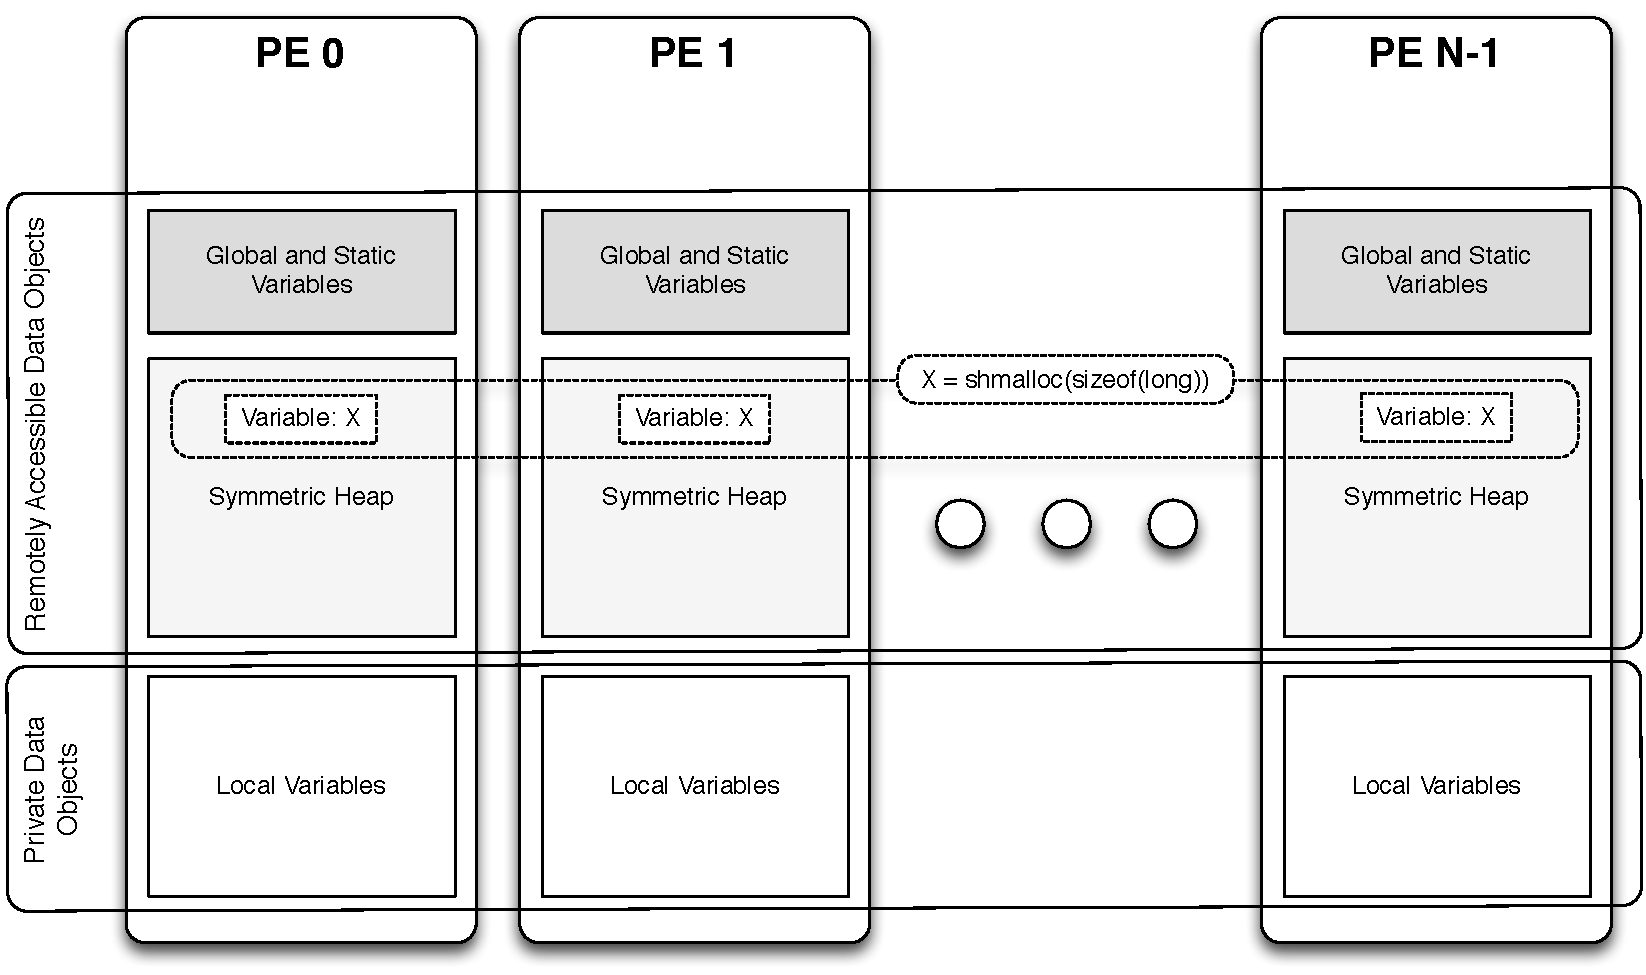
\includegraphics[width=0.95\textwidth]{diagrams/updated/mem_model}      
\caption{\OSH{} Memory Model}                                   
\label{fig:mem_model}                                               
\end{figure}      
An \openshmem program consists of data objects that are private to each \ac{PE} and data 
objects that are remotely accessible by all \ac{PE}s. Private data objects are stored in the local
memory of each \ac{PE} and can only be accessed by the \ac{PE} itself; these data objects
cannot be accessed by other \ac{PE}s via \openshmem routines. Private data objects
follow the memory model of \Clang{} or \Fortran{}. Remotely accessible
objects, however, can be accessed by remote \ac{PE}s using \openshmem routines.
Remotely accessible data objects are called \emph{Symmetric Objects}.
An object is symmetric if it has a corresponding object with the same
type, size and offset from an arbitrary memory address all \ac{PE}s. \emph{Symmetric objects } shall be accessible by any \ac{PE} via the \openshmem \ac{API}.  
In \openshmem{} the following kinds of data objects are symmetric:
\begin{itemize}
  \item \Fortran{} data objects in common blocks or with the  SAVE  attribute. These data objects	must not be defined in a dynamic shared object (DSO).
  \item Non-stack \Clang{} and \Cpp{} variables.   These  data	objects must  not  be defined in a DSO.
  \item \Fortran{} arrays allocated with \textit{shpalloc} 
  \item \Clang{} and \Cpp{} data allocated by \textit{shmalloc}
\end{itemize}       

%Symmetric Objects
%are static and global variables in \Clang{} and \Cpp, which are often allocated
%at the same address on all \ac{PE}s where the program is being executed
%(\emph{e.g.} in the ELF executable format). 
%See Figure \ref{fig:SymmetricHeap1}
%for an example of how Symmetric Memory Objects may be arranged in
%memory.
\openshmem routines (\textit{shpalloc} and \textit{shmalloc}) allow the creation of dynamically allocated \emph{Symmetric
Data Objects}. These objects are created in a special memory region
called the Symmetric Heap. The Symmetric Heap is created during the execution of a program at a location
determined by the implementation. The Symmetric Heap may reside on
different memory regions on the different \ac{PE}s. Figure~\ref{fig:mem_model} shows how \openshmem implements a \ac{PGAS} model 
using remotely accessible (\emph{Symmetric objects}) and private data objects. Symmetric data objects are stored in the symmetric heap or 
or in the global / static memory section of each \ac{PE}. Symmetric data objects can be allocated dynamically in the symmetric heap of each \ac{PE} using
a collective \FUNC{shmalloc} or \FUNC{shpalloc} memory allocation call.
     
%\openshmem specification does not require a particular memory layout; it is up to the implementation
%to decide how to implement the symmetric heap.  
%Objects that reside in the private address space can only be accessed by the \ac{PE} itself; these data objects
%cannot be accessed by other PEs via \openshmem routines. 